% The \documentclass command is the first command in a LaTeX file.
\documentclass{bsu-ms}
%\documentclass[project]{bsu-ms}  % for project reports

\pagenumbering{arabic}

\usepackage{graphicx}
\usepackage{algorithm}
\usepackage[noend]{algpseudocode}
%\usepackage{epstopdf}

\begin{document}

\subsection*{Eddie Davis and Mike Ramshaw}
\textbf{CS 530}\\
\subsection*{PA3: Lab Report (11/18/2016)}

\section*{1 Algorithm Description}

Massive scale text searching is one of the quintessential problems in the big data paradigm. It is characterized by short queries (e.g., a web search for "funny cat memes"), and that most of the source documents will not match those queries (i.e., matches are sparse) . Such searches are greatly accelerated by maintaining indexes. An inverted index is one in which the search words are the keys, and the values are identifiers for documents in the collection that contain those words. A document can be any body of text, either web page, book, paper, or other. Subsequent searches need only query the index rather than searching the entire collection.

The process for building an inverted index for a collection consists of parsing the documents, splitting on word boundaries (e.g., whitespace, punctuation, etc.), and building a lookup table where each word is linked to the set of documents wherein it can be found. A naive approach might be to parse each file by line, tokenize each line, and inserting the file name into an associative array of lists with tokens as keys. See Figure 1 for an inverted index example, and Algorithm 1 for a potential sequential implementation.

\begin{figure}[ht]
	\begin{center}
		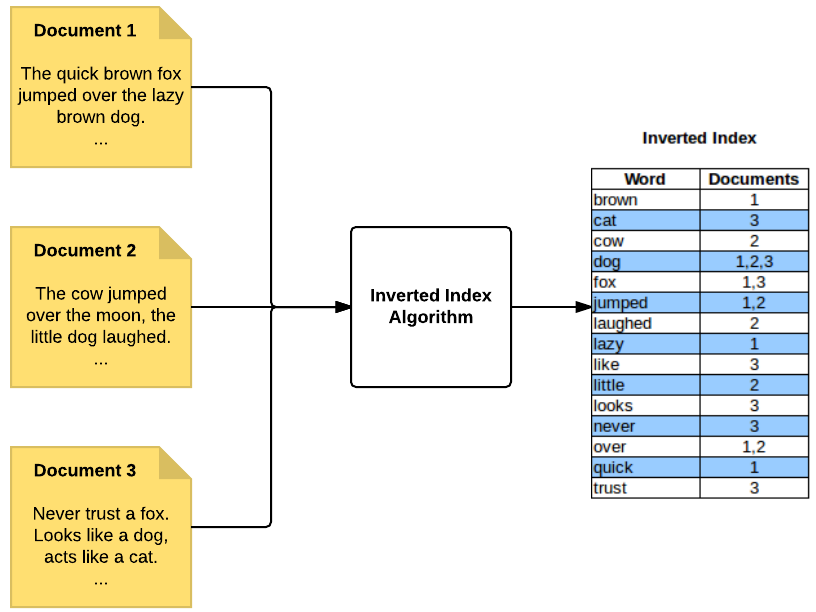
\includegraphics[scale=.6,keepaspectratio]{invertedindex.png}
	\end{center}
	\caption{Inverted index example for three sample documents.}
	\label{fig:fig1}
\end{figure}

\begin{algorithm}
\caption{Sequential Inverted Index }
\label{alg:alg1}
\begin{algorithmic}[0]
\Function{SequentialInvertedIndex}{$coll$}\Comment{Collection coll}
	\State $M \gets \texttt{new AssociativeArray}$
	\ForAll{$doc \in coll$}\Comment{Document doc}
		\ForAll{$word \in doc$}
		    \If{$word \notin M$}
   		        \State $M\{word\} \gets \texttt{new Set}$
		    \EndIf
		    
		\State $M\{word\}.add(doc.id)$
     	\EndFor
	\EndFor

   \State $F \gets \texttt{new File}$
    \ForAll{$word \in M$}
   		\State $F.write(F, M\{word\})$
    \EndFor
	
	%\Return $A$
\EndFunction
\end{algorithmic}
\end{algorithm}

\section*{2 Parallelization Approach}

MapReduce is a parallel programming model inspired by the \texttt{map} and \texttt{reduce} statements from functional programming languages. Problems are represented as sets of key-value pairs. A mapper component filters or sorts the data into a common key, and the reducer performs some summarizing operation on all the values containing that key. The Hadoop infrastructure allows these operations to be distributed across a large cluster in a massively parallel fashion.

The inverted index problem is a natural fit for the MapReduce paradigm, particularly for large sets of documents as a sequential search would be quite time intensive. The initial MapReduce implementation is described in Algorithm 2.

\begin{algorithm}
	\caption{MapReduce Inverted Index 1}
	\label{alg:alg2}
	\begin{algorithmic}[0]
		\Function{map}{$id, doc$}		
		\ForAll{$word \in doc$}		
		\State $\texttt{\textbf{emit}}(word, id)$
		\EndFor
		\EndFunction		

		\Function{reduce}{$word, [id_1, id_2, ..., id_n]$}		
		\State $output \gets ""$
		\ForAll{$id \in [id_1, id_2, ..., id_n]$}
		\State $output \gets output \| id$
		\EndFor
		\State $\texttt{\textbf{emit}}(word, output)$
		\EndFunction		
	\end{algorithmic}
\end{algorithm}

This algorithm is effective but results in redundant document IDs in the final output. The first improvement is to count the number of times each word occurs in a given document and emit that from the mapper class to eliminate the repetitive output. This implementation takes advantage of the in-mapper combiner design pattern. The \texttt{setup} method initializes an associate array, a Java \texttt{HashMap} specifically. The \texttt{map} method updates the counter for each word in the array. Finally, the \texttt{cleanup} method emits the word, count pairs for each document.

The \texttt{reduce} method is responsible for collecting the count, document pairs for word, combining them into a single output, and emitting them. See Algorithm 3.

\begin{algorithm}
	\caption{MapReduce Inverted Index 2}
	\label{alg:alg3}
	\begin{algorithmic}[0]
		\Function{setup}{}		
			\State $M \gets \texttt{new AssociativeArray}$
		\EndFunction
		
		\Function{map}{$id, doc$}
		\ForAll{$word \in doc$}		
		\If{$word \notin M$}
		\State $M\{word\} \gets 0$
		\EndIf
		
		\State $M\{word\} \gets M\{word\} + 1$
		\EndFor
		\EndFunction		
		
		\Function{cleanup}{}
		\ForAll{$word \in M$}
		\State $\texttt{\textbf{emit}}(word, M\{word\})$
		\EndFor
		\EndFunction
		
		\Function{reduce}{$word, [(c_1, id_1), (c_2, id_2), ..., (c_n, id_n)]$}		
		\State $output \gets ""$
		\ForAll{$(c, id) \in [(c_1, id_1), (c_2, id_2), ..., (c_n, id_n)]$}
		\State $output \gets output \| c \| id$
		\EndFor
		\State $\texttt{\textbf{emit}}(word, output)$
		\EndFunction		
	\end{algorithmic}
\end{algorithm}

The last improvement to the algorithm is to sort the document IDs in the reducer output by the count in reverse order, such that the files with the greatest number of matches appear first. This is accomplished by implementing a custom writable class called \texttt{FileCountWritable}. This class is emitted by the mapper and implements the \texttt{compareTo} method, allowing the reducer to easily sort the document IDs by count.

\section*{3 Experimental Setup}

The run times of the sequential version of the program (\texttt{sequential-bucketsort}) are the baseline (control) for this experiment, or the $T_s(n)$ for the speedup calculations. The experimental groups will run the parallel version (\texttt{parallel-bucketsort}) with processes \textit{p} $\in$ (2, 4, 8, 16), and iterations \textit{n} $\in$ (1E9, 2E9, 5E9). In order to ensure that the code performs well on different data distributions, three random seed values $s \in$ \{6764, 445455, 2876533 \} are included, with the mean run time reported.

The experiments were performed on the \texttt{onyx} Fedora Linux cluster. Each node  contains an Intel(R) Xeon(R) E31225 processor with four cores clocked at 3.10 GHz. The CPUs include 6144 KB of level three (L3) cache shared by the four cores, 256 KB of level two (L2) cache, and 64 KB of level one (L1) cache per node. Each node has 8 GB of main memory (DRAM) onboard.

\section*{4 Experimental Results}


\section*{5 Conclusions}



\end{document}
